\section{Introduction}
Business Process Model and Notation (BPMN) \cite{BPMN20}, also known as Business Process Modeling Notation, is a standard graphical representation of business process models. BPMN bridges the gap between
visualization of the business processes and their actual implementation by providing an understandable notation for both business stakeholders and technical experts.

BPMN is based on flowcharting techniques. It allows modeling complex business processes using its diverse set of control structures, which covers concepts such as sequencing, repetition, choice, concurrency, messaging, failure, transactions, etc. BPMN has an expressive notion to define events and to associate triggers to the defined events. Furthermore, it provides means to form reusable units out of a set of elements. 

The first version of BPMN is developed by the Business Process Management Initiative (BPMI) in 2004. In 2005, BPMI and the Object Management Group (OMG) merged. BPMN is maintained by OMG since then. In 2006, the BPMN specification was adopted as an OMG standard. In 2011, the final edition of BPMN 2 specification was released.

BPMN 1.2 presents a notation for modeling business processes and informally expresses the semantics of the modeling primitives. This leads to ambiguity and confusions in interpretation of a process. For instance, the authors in \cite{viciouscirc} present a deadlock situation called \emph{vicious circle} that is caused by using convergent \emph{inclusive gateway}s. This is a class of situations where two \emph{inclusive gateway}s are connected 
 in a cyclical way. % However, in spite of these changes the vicious circle example may still exhibit race-conditions in BPMN 2 [72]????. 
 Moreover, BPMN 1.2 specification provides no details on model serialization format.

BPMN 2, the biggest revision of BPMN so far, presents a formal definition in terms of a meta-model, that is a formal definition of the constructs and their relations in a valid model. The meta-model specifies a serialization format that enables model exchange among different BPMN 2 tools. 
In the context of modeling elements, BPMN 2 offers the following enhancements over previous versions:

\begin{itemize}
\item It expands the set of BPMN gateways with \emph{exclusive} and \emph{inclusive} event-based gateways.
\item It enriches the set of activities by adding \emph{business rule task}, \emph{sequential multi-instance} activity, \emph{event sub-process} that handles events occurring in bounding \emph{sub-process}, and
\emph{call activity} that invokes a global \emph{sub-process}.
\item It enhances \emph{event}s by introducing \emph{escalation}, and \emph{complex events}, and the concept of \emph{interrupting} and \emph{non-interrupting} events.
\end{itemize}

%\item artifacts (data objects)???
%\item It offers four types of diagrams for modeling business processes:
%\begin{itemize}
%\item[-] Process diagrams, which They
%
%\item[-] Orchestration They represent a specific business or organization?s
%view of the process. It describes how a single business entity (i.e., a
%process participant, such as a buyer, seller, shipper, or supplier) goes
%about things. A BPMN diagram may contain more than one
%orchestration. If so, each orchestration appears within its own container
%- called a Pool. Each Pool can only represent one participant.
%\item[-] CollaborationIt is merely a collection of participants and their
%interaction.
%\item[-] Choreography They
%represent the expected
%behavior between two or
%more business participants.Choreographies Expand BPMN to allow model orchestrations and choreographies as stand-alone or integrated models.
%\item[-] ConversationThe logical
%relation of message
%exchanges
%\end{itemize}
%\end{itemize}

Although BPMN 2 provides an explicit execution semantic, the semantics are expressed in  informal fashion. This leaves rooms for interpretation for a number of issues such as deadlocks and race conditions. 

%In this chapter we give an informal description of BPMN 2, and introduce a running example
%Figure 2.1: Our subset of BPMN elements
%In this thesis we consider the subset of BPMN shown in Figure 2.1. Some BPMN elements have been
%omitted from this subset due to one of the following reasons.
%1. The element is used specifically to express data flow or transactional behaviour.
%2. The element may be semantically expressed using a combination of elements in the subset shown
%in Figure 2.1.
%In this thesis we consider synchronous communications between elements in a BPMN diagram. We do
%not consider transactional behaviour: we believe that transactional behaviour should be studied with a
%formal modelling language, such as Compensating CSP [BHF05], that has transaction and compensation
%built into its syntax and semantics. Similarly, we do not consider data flow behaviour: data flow
%communications are asynchronous and should be studied with a formal modelling language, such as
%Data-Flow Sequential Processes [Jos05], that has asynchronous interactions as its primitives. In the
%remaining section we describe the elements in this subset and justify why an element or a particular
%behaviour of an element is not selected.
%of elements that come before the source of the gateway?s incoming sequence flows at runtime [DGHW07].

In this chapter, we provide an overview to BPMN. We also present examples of process models containing semantical errors.

\section{BPMN 2 elements}
A BPMN diagram consists of a number of elements that fall into the categories of \emph{flow objects}, \emph{connecting object}s, \emph{swimlane}s, and \emph{artifacts}. A flow object can be
an \emph{event}, a \emph{gateway}, or an \emph{activity}. 

\subsection{Connecting objects}
\emph{Connecting objects} are used to connect the other BPMN elements: 
\begin{itemize}
\item \emph{Sequence flow}s represent the occurring order of processes in a business model. 
\item \emph{Message flow}s are used to exchange messages between process participants. 
\item \emph{Association flow}s associate modeling elements to each other. For instance, a \emph{compensation task} is associated to its task via an association flow.
\end{itemize}

%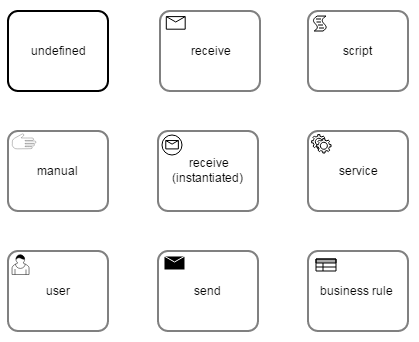
\includegraphics[width=\textwidth]{img/IC-BPMN-business-rules-c} 
%
%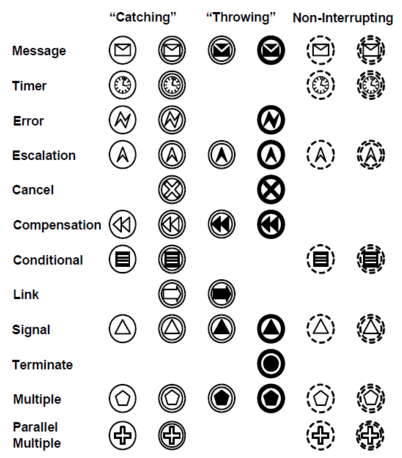
\includegraphics[width=\textwidth]{img/IC-BPMN-event-sub-processes-c} 
%
%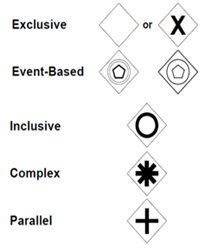
\includegraphics[width=\textwidth]{img/IC-BPMN-parallel-c} 

\subsection{Events} 
Events represent triggers occurring during execution of business processes. Events usually have a \emph{cause} or a \emph{result}. The representation of an \emph{event} is a circle wherein internal markers are placed to denote triggers or results. 
Based on the time that events affect the flow, they fall into three categories: %%% \emph{start}, \emph{intermediate}, and \emph{end} events
%\vspace*{1cm}
%\begin{itemize}
%\item  
%
\includegraphics[height=3ex]{img/bch-evstart} 
%\emph{Start events}, which start a process;
%
%\item 
%
\includegraphics[height=3.5ex]{img/inter} 
%\emph{Intermediate events}, which occur between start and end of a process; 
%
%\item  
%
\includegraphics[height=3ex]{img/bch-eventend}
%\emph{End events}, which terminate a process.
%\end{itemize}

\begin{table}[H]
 \centering
     \begin{tabular}{ cl}%p{.5\textwidth}}
     %\hline
    % &\\
     \raisebox{-.1cm}{\hspace{-1cm} {
\includegraphics[width=0.04\textwidth]{img/bch-evstart}  }}
      &%\hspace*{-6mm}
      \emph{Start events}, which start a process;
      \\ &\\ %\hline
   %   & \\
     \raisebox{-.1cm}{\hspace{-1cm} 
\includegraphics[width=0.043\textwidth]{img/inter}  }
      & %\hspace*{-6mm}
\emph{Intermediate events}, which occur between start and end of a process;      \\% &\\ % \hline
& \\
 %\cmidrule(r){1-1}\cmidrule(lr){2-2}\cmidrule(l){3-3}
     \raisebox{-1mm}{\hspace{-1cm} 
\includegraphics[width=0.04\textwidth]{img/bch-eventend}  }
& %\hspace*{-.6cm}
\emph{End events}, which terminate a process.
\\ %& \\ %\hline
      \end{tabular}
\end{table}
      
\noindent
Each time a process receives a new start event trigger, a new instance of the process begins to execute. Therefore, a process may have many process instances. Start events and intermediate events are \emph{catching}, meaning that they catch a trigger in order to occur.
End events and some of intermediate events are \emph{throwing} as they throw a result. Compared to the passive nature of catching events, throwing events are \emph{active} as they trigger themselves rather than waiting for a trigger to 
take place.

The following intermediate events can attach to the boundary of an activity: \emph{message}, \emph{timer}, \emph{error}, \emph{compensation}, and \emph{signal}. %TODO all of this? to check
In this case, they can only occur while the surrounding activity is active. \emph{Boundary event}s can either be interrupting or non-interrupting. %fashion, represented by solid and dashed boundaries, respectively. %???TODO 

Interrupting events stop the execution of the activity and direct the flow out of the boundary event, while non-interrupting events do not interfere with the execution of the activity. Instead, they start the flow out of the boundary event in parallel. Another difference is that non-interrupting events can occur several times while the surrounding activity is running. 

Following is the list of event types in BPMN 2:

\begin{table}[H]
\centering
\begin{tabular}{ cp{10cm} }
%\hline&\\
 \raisebox{-.4cm}{\hspace{-1.2cm}
 
\includegraphics[height=3ex]{img/bch-evstart}} &
 A \emph{none} event has no defined trigger. It can indicate a start point, a state change or a final state. Each process can only have one \emph{none start event}.
 \\  %&\\ %\hline
 & \\
  \raisebox{-.28cm}{\hspace{-1.2cm} 
\includegraphics[height=3ex]{img/bch-eventmsg}} &
 A \emph{message} event is used to model exchange of messages. A message has a specific receiver. 
\\  %&\\ %\hline
& \\
 \raisebox{-.38cm}{\hspace{-1.2cm} 
\includegraphics[height=4ex]{img/bch-signal}} &
A \emph{signal} is broadcasted between processes. It differs from message in that a message has a specific target, but a signal is broad-casted.
A  thrown signal can be caught multiple times.%who receives it?
\\ %&\\
%\hline
& \\
 \raisebox{-.2cm}{\hspace{-1.2cm}
%
\includegraphics[height=3ex]{img/bch-eventtimer}  

\includegraphics[height=3ex]{img/bch-int-timer-event} }&
A \emph{timer} event indicates a waiting time within the process. A timer trigger can be a specific date/time value or a duration. 
\\ &\\
 \raisebox{-.3cm}{\hspace{-1.2cm}
\includegraphics[height=3ex]{img/bch-eventrule}} &
 A \emph{conditional} event occurs when a business condition becomes true.\\ 
 %%%%%%%%%%%%%
  &\\
  \raisebox{-.5cm}{\hspace{-1.2cm} 
\includegraphics[height=3ex]{img/bch-eventlink} } &
A \emph{link} is a mechanism for connecting two sections of a process. 
 %TODO Link Events can be used to create looping situations or to avoid long Sequence Flow lines. Link Event uses are limited to a single Process level (i.e., they cannot link a parent Process with a Sub-Process).
%It is connected by association links rather than sequence flows. 
 A throwing link event is used at the exit point, while a catching link event as the entrance point. 
%Link is used only as intermediate event. 
 Using link helps keeping the model clean and prevents spaghetti models.
%The Link Intermediate Events are only valid in Normal Flow, i.e. they may not be used on the boundary of an Activity. 
\\ & \\
\raisebox{-.5cm}{\hspace{-1.3cm} 
\includegraphics[height=3ex]{img/bch-eventcancel} } &
A \emph{cancel} event is always used with a transaction sub-process. It indicates that the transaction should be canceled. A cancel event triggers a cancel intermediate event attached to the sub process boundary. %In addition, it will indicate that a transactional protocol cancel message should be sent to any entities involved in the transaction. 
%TODO The Cancel Intermediate Event can only be used when attached to the boundary of a Transaction Sub-Process. 
% It can be triggered; if the cancel transaction is reached in the process or a cancel event is received. Like Error event it will always interrupt the current Sub Process. It cannot be marked as non-interrupting cancel event
\\ %& \\ %\hline  
     %\hline 
%Catching or throwing named errors
%Given the nature of Errors, an Event Sub-Process with an Error trigger will always interrupt its containing Process.
%Used as catching it can be only used as attached intermediate event, as throwing it can only indicates the end of a process.
%\end{tabular}
%\begin{table}[!h]
     %\begin{center}
 %    \begin{tabular}{ lp{11.2cm} }
 &\\
  \raisebox{-.2cm}{\hspace{-1.5cm} 
\includegraphics[height=3ex]{img/bch-eventterminate}} &
A \emph{terminate} event  indicates that all activities in the process should be immediately ended. In this case, the process is ended without compensation or event handling. 
%\end{tabular}
\\ %& \\
%\hline
%\noindent
%\hspace*{-.2cm}
%\begin{table}[!h]
     %\begin{center}
     %\begin{tabular}{ lp{11.2cm} }
     & \\
\raisebox{-.5cm}{\hspace{-1.4cm} 
\includegraphics[height=3ex]{img/bch-eventcomp}  }&
 %A compensation event does not interrupt the process, since the process has to be completed before this event can be triggered.
A \emph{throwing compensation} event indicates that a compensation is needed. A catching compensation event states that a compensation will occur when the event is triggered.
%TODO There are two mechanisms that can signal the cancellation of a Transaction:
%TODO 1) A Cancel End Event is reached within the transaction Sub-Process. A Cancel End Event can only be used within a transaction Sub-Process.
%TODO 2) A cancel Message can be received via the transaction protocol that is supporting the execution of the Transaction Sub-Process.
%TODO Hazard: This means that something went terribly wrong and that a normal success or cancel is not possible. 
%Error Intermediate Events are used to show Hazards. When a Hazard happens, the Activity is interrupted (without compensation) and the flow will continue from the Error Intermediate Event.
%
%But it is possible that one of the Participants can end up with a problem that causes a Cancel or a Hazard. In this case, the flow will then move to the appropriate Intermediate Event, even though it had apparently finished successfully.
%A cancel EndEvent is only allowed in a transaction sub-process. An end event must be present when a start event is used in the same process level.
%Attached compensation events connect to compensation tasks by association links rather than sequence flow.
All other boundary events occur only while the activity that they are attached to is active. In contrary, an attached compensation takes place only if the process triggers a compensation and if the activity to which compensation is attached has been completed successfully. %TODO rephrase
\\ & \\ %\hline
\raisebox{-.2cm}{\hspace{-1.4cm} 
\includegraphics[height=3ex]{img/bch-event5zeli} } &
A \emph{multiple} event summarizes several events with a single event. A catching multiple event occurs if at least one of its specified events occurs. However, a throwing multiple triggers all the defined events.
\\% & \\ %\hline
%& \\
    \end{tabular}
\end{table}

\begin{table}[H]
\centering
\begin{tabular}{ cp{10cm} }
%\hline&\\
 \raisebox{-.5cm}{\hspace{-1cm} 
\includegraphics[height=3ex]{img/bch-eventplus}}  & %\hspace{-.6cm}
A \emph{parallel multiple} event, which is  added in BPMN 2, is  a supplement to multiple event. A parallel multiple event is only catching. It indicates that all of the defined events are required in order to trigger this event.
%TODO BPMN 2 introduces the parallel multiple event, which has inclusive behavior, meaning that all related events are required in order to trigger the shape.   There is no throwing type for this shape, because a parallel throwing multiple event would probably raise more questions than it solves http://www.processmodeling.info/posts/highlights-from-bpmn-2-0-new-event-types/
\\ %& \\ %\hline
& \\
  \raisebox{-.5cm}{ \hspace{-1cm}  
\includegraphics[height=3ex]{img/bch-eventescalation}} &
\emph{Escalation} is new in the BPMN 2 specification. An escalation event is used to trigger a path in middle of a process flow that requires involvement of a higher responsibility.
%TODO http://www.moonstarinc.com/2013/04/bpmn-2-0-intermediate-event/
 %TODO However, it’s important to note that both start (interrupting/non-interrupting) and both intermediate types can only be used with sub-processes. Only the throwing shapes can be used within normal sequence flow.   This implies that escalation can only be thrown from within a subprocess that has a catching shape.  The intermediates are used on the subprocess border, whereas the start types are used within the subprocess.  Note that you should review non-interrupting events in my previous post for more details on how non-interrupting events work.
 \\ %& \\ %\hline
\end{tabular}
\end{table}

Based on the types, event triggers are forwarded in five different strategies:
\begin{itemize}
\item \emph{Publication}: A published trigger can be caught by any catching event that matches the trigger within any scope where it is published. \emph{Message} and \emph{signal} events triggers are forwarded this way. 

Messages are created 
out of the pool wherein they are published. In case that a message should be received by a specific process instance, the particular instance in referred by the message.

Signals are created inside the pool wherein they are published. In general, signals are used to broadcast within and across processes, pools, and process diagrams.
\item \emph{Direct Resolution}: The timer and conditional triggers are thrown implicitly.  These triggers wait for a defined time or a specific condition to trigger the related catch event, respectively.

\item \emph{Propagation}: A propagated trigger is forwarded from its origin to the innermost enclosing level that has an attached catching event that matches the trigger. Instances of events that propagate are \emph{error} and \emph{escalation}.

Unlike error triggers that are critical and suspend execution, escalations are non-critical and allow execution to proceed normally. If there is no catching event found for an error or an escalation trigger, the trigger is unresolved.

\item \emph{Cancellation}: When a \emph{cancellation} occurs, all running activities terminate and all activities  in the sub-process wherein cancellation applies are compensated, if they are completed successfully.
In case that the sub-process is a transaction, it needs to be rolled back. 
\item \emph{Compensation}: A successfully completed activity is \emph{compensated} by its compensation handler, which is either user-defined or implicit. In latter case, the compensation handlers of the enclosed activities are invoked in the reverse order of their execution. If an activity has not completed successfully, nothing happens and no error is raised.
\end{itemize}

\subsection{Activities}
%Since a Reo network focuses on coordination aspects of the modeled system, rather than its functional behavior,
%we translate BPMN tasks and sub-processes to black-boxes whose collaboration is coordinated by
%Reo channels.
An activity describes the type of work that needs to be done. An activity is either a task, a sub-process, or a transaction.
BPMN represents the activity in a high-level of abstraction. It is not the BPMN responsibility to describe the activity details. %Tables \ref{table:compe1} and \ref{table:compe} describe BPMN 2 activities.

\noindent
%\hspace*{-.2cm}
\begin{table}[H]
\centering
\begin{tabular}{ cp{9.5cm} }
%\hline
%& \\
  \raisebox{-.85cm}{ 
\includegraphics[width=10ex]{img/bch-task-khali}} &
\emph{Tasks}, which are atomic activities have several types:
%\begin{itemize}
\\ & \\
%\hline
%& \\
 \raisebox{-.85cm}{ 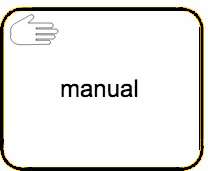
\includegraphics[width=10ex]{img/bch-task-man}} &
A \emph{manual task} is a task that is performed manually.
\\ %&\\
%\hline
& \\
 \raisebox{-.85cm}{\hspace{.1cm}  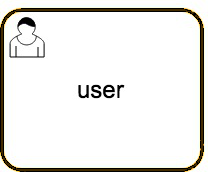
\includegraphics[width=10ex]{img/bch-task-usr} } &
A  \emph{user task} is performed by a person with assistance of automation.\\ &
\\ 
%\end{tabular}
%\end{table}
%
%\noindent
%\hspace*{-.2cm}
%\begin{table}[H]
%\centering
%\begin{tabular}{ cp{10cm} }
%\hline
%& \\
%\hline &\\
\raisebox{-.85cm}{ 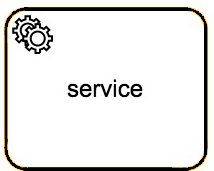
\includegraphics[width=10ex]{img/bch-task-src} } &
 \emph{Service tasks} are services such as web services or automated applications. \\ %& \\
 %\hline
 %\end{tabular}
 %\end{table}
 %
 %\noindent
%\hspace*{-.2cm}
%\begin{table}[!h]
     %\begin{center}
  %   \begin{tabular}{ |c|p{10cm}| }
   %  \hline
	     &\\
 \raisebox{-.85cm}{\hspace{-.15cm}
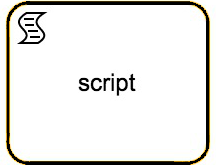
\includegraphics[width=10ex]{img/bch-task-scrp}} &
A \emph{script task} is executed by a business process engine. 
\\% & \\
%\hline
& \\
	     \raisebox{-.85cm}{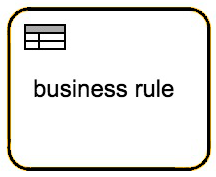
\includegraphics[width=10ex]{img/bch-task-bz}} &
\emph{Business rule tasks} are introduced in BPMN 2. They are performed by business rule engines.
\\ & \\
%\hline
%&\\
  \raisebox{-.85cm}{ 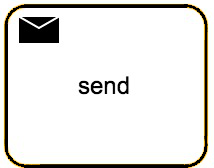
\includegraphics[width=10ex]{img/bch-task-snd} }&
 A \emph{send task} is a simple task with an outgoing message flow, which is used for sending messages. The task is completed after the message is sent. \\ & \\
 %\hline
 %& \\
 \raisebox{-.85cm}{\hspace{0cm} 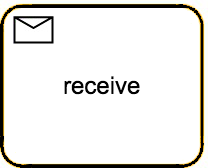
\includegraphics[width=10ex]{img/bch-task-rec} }&
A \emph{receive task} is a simple task with an incoming message flow, which waits for a message to arrive. Once it receives the message, the task is completed. 
%\\ &
\\
%\hline
%\end{itemize}
\end{tabular}
%\caption{BPMN 2 tasks}
%\label{table:compe1}
\end{table}

A \emph{sub-process} captures a set of activities, gateways, and flows within a single activity. It hides or reveals details of business process based on being expanded or collapsed, which is denoted using a plus sign at the bottom of the sub-process.
A sub-process may only begin with a \emph{none start} event and end with a \emph{none end} event.


 \noindent
%\hspace*{-.2cm}
%\begin{table}[!h]
     %\begin{center}
%\hspace*{-.2cm}
\begin{table}[H]
\centering
\begin{tabular}{ cp{10cm} }
     %\hline
      %       &\\
 \raisebox{-1cm}{\hspace{-1cm} 
\includegraphics[width=10ex]{img/bch-xaction}} &
A \emph{transaction} is a sub-process that all of its enclosed activities constitute a logical unit of operation, meaning that all the activities must be completed successfully, and if one fails, all of them need to be compensated. %TODO Transactions are differentiated from expanded sub-processes by being surrounded by a double border.
\\ & \\ %\hline
%\end{tabular}
%\end{table}
%
%\noindent
%\begin{table}[t]
%\centering
     %\begin{tabular}{ |c|p{9cm}| }
  %   \hline & \\
  \raisebox{-2cm}{\hspace{-.9cm}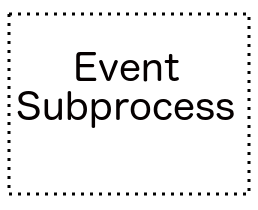
\includegraphics[width=10ex]{img/bch-eventsub} }&
\emph{Event sub-process} are introduced in BPMN 2. An event sub-process behaves like a boundary event, but it resides inside a process or a sub-process rather than on their boundaries. 

An event sub-process can be considered as an optional sub-process that occurs when its start event is triggered. 

Similar to boundary events, an event sub-process may interrupt the containing process or run in parallel in a non-interrupting fashion, depending on the type of its start event. 

In addition, it is allowed to have only one start event that is non-empty. The event types that can be used as a start event for an event sub-process are: \emph{message}, \emph{conditional}, \emph{signal}, \emph{timer}, \emph{escalation}, \emph{error}, \emph{multiple}, and \emph{parallel-multiple}. As mentioned, the only way to run an event sub-process is by triggering its start event. As a result, no incoming or outgoing sequence flow can connect to an event sub-process.
\\ %& \\ \hline
\end{tabular}
%\caption{BPMN 2 transaction and event sub-process}
%\label{table:compe}
\end{table}

In BPMN 1.2, there are two types of sub-processes: \emph{embedded} and \emph{reusable}. BPMN 2 sub-processes are inherently embedded. They can only be reused if they are defined globally and are referenced by call activities.

An embedded sub-process can only contain a \emph{none start} event. It cannot have  other types of start events such as timers or messages. %It also cannot have any pool or lane. 

Furthermore, an embedded sub-process can only be found inside a process to which it belongs. A global sub-process, on the other hand, can reside within different processes. %An example of such sub-processes that is used over and over is the procurement of an item due to a customer order.
%rewrite beshe
%A sub-process is instantiated when it is reached by a sequence flow token. The sub-process has either a unique empty start event, which gets a token upon instantiation, or it has no start event but activities and gateways without incoming sequence flows. In the latter case all such activities and gateways get a token. A sub-process must not have any non-empty start events.
%If a sub-process is collapsed, then we treat it as a black box and map it to a FIFO$_1$ channel with its ends attached to nodes for further connections. A sub-process may have intermediate and boundary events attached to it, which we deal with their mapping in the section corresponding to the events. For an expanded sub-process, we map the elements inside the sub-process as given in the relevent mappings.   
%may A as shown in FIgure ??? 
%input -> (node) -> fifo1  -> 

In BPMN 2, reusable task and sub-processes are invoked using a \emph{call activity}. 
 According to the BPMN 2 specification \cite{BPMN20}, a call activity in BPMN 2 corresponds to the BPMN 1.2 reusable sub-process, while a sub-process in BPMN 2 corresponds to the BPMN 1.2 embedded sub-process.


A transaction has three possible outcomes:

 \begin{itemize}
\item  All the activities finish \emph{successfully}. In this case, the process proceeds with the normal flow. 
\item  In case of a \emph{failure}, the compensation tasks associated to the successfully completed activities execute. The process continues through the cancel intermediate event.
\item  In case that an \emph{unexpected error} takes place, the sub-process activities are interrupted without any compensation. The process then proceeds with the intermediate error event.
\end{itemize}

%The mapping should provide a mechanism for compensation tasks to be executed upon the occurrence of an error, if their corresponding tasks have already been executed. 
%In addition, it should provide a way for the tasks with error events to propagate the error and cancel the transaction.
%TODO Our approach in mapping transactions differs from ??? in that ??? cosiders external cancel %and commit messages being sent to a transaction. Thus, ???  does not take the internal errors %into consideration, while in BPMN 2 the transactions are canceled due internal errors.A transaction is canceled, if an execution reaches the cancel end event. In that case, all executions are terminated and removed. A single remaining execution is then set to the cancel boundary event, which triggers compensation. After compensation is completed, the transaction sub-process is left using the outgoing sequence flows of the cancel boundary event.
%A transaction is ended by a hazard, if an error event is thrown, that is not caught within the scope of the transaction sub-process. 
%\end{itemize}%http://help.bizagi.com/bpmsuite/en/index.html?understandingtransactionalsubprocesses.htm

An activity can be annotated using different \emph{markers} that indicate the nature of the activity. The markers are as follows:
\begin{itemize}
\item The \emph{loop} marker indicates that the attached activity executes multiple times until the loop condition holds. The condition can be evaluated either in the beginning or in the end of the activity depending on a specific attribute of the activity.

\item A \emph{compensation} marker is used to undo a completed activity.% If a compensation marker is marked on a task it will reverse the previous task or that belong in a single transaction. 
\item A \emph{sequential multi-instance} marker defines an activity that has multiple instances created sequentially. The number of instances to be instantiated is either defined as an attribute of the activity or as the cardinality of input data items.%TODO rephrase
%We map a sequential multiple instance activity as figures above, if the number of instances are defined and if it depends on the input, respectively. 
%Figure ?? shows our mapping for parallel multiple instance in the former case. However, currently there is no mechanism for a Reo network to dynamically include more elements, therefore we skip the later case for parallel muliple instance.
\item A \emph{parallel multi-instance marker} represent activities that can be executed  in parallel as multiple instances. Each instance can have a different set of input parameters.
\item An \emph{ad-hoc marker} is used to represent an activity, whose inner tasks have no required order. Each task can start at any time.  There is no dependency among the activities.
%This marker is not frequently used in business process diagrams. But, it is useful if you are representing human behavior or activities which can perform any available task.
\end{itemize}

%(This also applies if the error is caught on the boundary of the transaction sub-process.) In this case, compensation is not performed.
%%http://www.bpm-guide.de/2012/03/02/activiti-5-9-introduces-bpmn-compensation-and-transactions/
%%Transaction: coordinates a set of activities have to be successfully completed. The possible transactional protocols that a transaction
%%might follow are: compensation, cancellation, and error. ???
%%?? and natltr??? suggest Reo translation for exception handling?? and BPMN transactions. However, in both case they consider the error message coming from outside of the sub-process that contains the transaction. However, according to BPMN2 ?? documentation, the internal tasks of the sub-process initiate the error message which triggers the associated compensation task. And afterwards, the error signal is sent out of the sub-process. Bases on this explanation, the followings are our Reo mapping for BPMN2 transaction:
%%Cancellation event, which enables an exception flow for the containing process is triggered when all the compensation activities are done.
%%The last result ??? of a transaction is error, which an unexpected situation occurs for which no covering procedure is defined. jaye event inja nist???
%The followings are our mapping for transactions. Notice that propagation for error is mainly needed for parallel / concurrent flows as shown in Fig??. In case, the flow is solely sequential, the mapping is simpler as shown in Fig ??   
% \subsection{jadid}
% A Business Process Diagram can be made up of a set of (semi-) independent components, which are shown as
% separate Pools, each of which represents an orchestration Process. There is not a specific mapping of the diagram
% itself, but rather, each of these orchestration Processes maps to an individual Reo module.
%
% Not all BPMN orchestration Processes can be mapped to Reo in a straight-forward way. That is because BPMN
% allows the modeler to draw almost arbitrary graphs to model control flow, whereas in Reo, there are certain
% restrictions such as control-flow being either block-structured or not containing cycles.????? %For example, an unstructured loop
% %cannot directly be represented in Reo.
%
% %To map a BPMN orchestration Process to Reo it MUST be sound, that is it MUST contain neither a deadlock nor
% %a lack of synchronization. A deadlock is a reachable state of the Process that contains a token on some Sequence
% %Flow that cannot be removed in any possible future. A lack of synchronization is a reachable state of the Process where
% %there is more than one token on some Sequence Flow. For further explanation of these terms, we refer to the literature.
% To define the structure of BPMN Processes, we introduce the following terminology. The Gateways and
% the Sequence Flows of the BPMN orchestration Process form a directed graph. A block of the diagram is a
% connected sub-graph that is connected to the rest of the graph only through exactly two Sequence Flows: exactly one
% Sequence Flow entering the block and exactly one Sequence Flow leaving the block. A block hierarchy for a
% Process model is a set of blocks of the Process model in which each pair of blocks is either nested or disjoint and
% which contains the maximal block (i.e., the whole Process model) A block that is nested in another block B is also
% called a subblock of B (cf. Figure 14.1). Each block of the block hierarchy of a given BPMN orchestration Process has
% a certain structure (or pattern) that provides the basis for defining the Reo mapping.
\subsection{Gateways}
Gateways manage the control flows within a process or sub-process by specifying the interaction among sequence flows as they converge and diverge. The list of BPMN 2 gateways follows:

%\vspace*{.2cm}
\noindent
\begin{table}[th]
\centering
     \begin{tabular}{ cp{10.5cm} }
     %\hline
%& \\
 \raisebox{-.6cm}{  
\includegraphics[height=4.8ex]{img/bch-gateway}} &
%
\includegraphics[height=5ex]{img/bch-eventexc} 
\emph{Data-based exclusive gateway}s are used to create alternative paths based on the conditions that are set on the incoming data flow. A diverging exclusive gateway, also called \emph{decision}, routes the incoming flows to one of the mutually exclusive alternative outgoing flows. A converging exclusive gateway directs one of its incoming flows to its only outgoing flow.
\\
%& \\
 %\hline
 & \\
  \raisebox{-.6cm}{ 
\includegraphics[height=5ex]{img/bch-eventinclu} } &
\emph{Data-based inclusive gateway}s create alternative but also parallel paths within a process flow. A diverging inclusive gateway directs its incoming flow to one or more outgoing flows based on conditions. A converging inclusive gateway, on the other hand, awaits incoming flows to complete.
%Unlike the Exclusive Gateway, all condition Expressions are evaluated
%The true evaluation of one condition Expression does not exclude the evaluation of other condition Expressions
%All Sequence Flows with a true evaluation will be traversed by a token
%\\ &
\\ % \hline
 & \\ \raisebox{-.6cm}{ 
\includegraphics[height=4.8ex]{img/bch-gwplus} }&
\emph{Parallel gateway}s are used to create and also to combine parallel flows. A diverging parallel gateway creates parallel flows, while a converging one merges the incoming flows into one outgoing flow.
\\ &
\\ %\hline & \\  
\raisebox{-.5cm}{ %
\includegraphics[height=5ex]{img/bch-gwpanjzeliicircle} 
\hspace{-.2cm} 
\includegraphics[height=5ex]{img/bch-panjzeliidodayare}} &
\emph{Event-based gateway} routes based on occurrence of events rather than on data. In addition to events, it also works with receive message task. An event-based gateway is always followed by catching events or receive tasks.
%The Event-Based Gateway represents a branching point in the Process where the alternative paths that follow the Gateway are based on Events that occur
%This is opposed to the evaluation of Expressions using Process data (as with an Exclusive or Inclusive Gateway which are Data Based)
%A specific Event, usually the receipt of a Message, determines the path that will be taken
%Basically, the decision is made by another Participant, based on data that is not visible to Process, thus,
%requiring the use of the Event-Based Gateway.
\\ & \\ 
%\hline   & \\ 
\raisebox{-.5cm}{ 
\includegraphics[height=5ex]{img/bch-eventplusdayere} } &
A \emph{parallel event-based Gateway} is similar to a parallel data-based gateway with the difference that it depends on occurrence of events rather than on data.
\\ & \\ %\hline  & \\
  \raisebox{-.5cm}{ 
\includegraphics[height=5ex]{img/bch-eventsetare} } &
A \emph{complex gateway} models complex synchronization behavior. An expression is used to describe the behavior of the gateway. %BPMN 2 2offers updates on the event gateways. In BPMN 1.x event gateways may initiate a process. However, there was no visual indication for such case. BPMN 2 provides a notational difference between the event gateways that initiate a process and those that do not. %The Event Gateway that does not initiate a Process maintains the original internal marker that looks like a Multiple Intermediate Event (see left Gateway in Figure 12). The Event Gateway that does initiate a Process now has an internal marker that looks like a Multiple Start Event (see middle Gateway in Figure 12). This notational distinction accurately reflects the behavior of the two Event Gateway variations.
%Both the initiating and non-initiating versions of the Event Gateway direct the Process flow exclusively. This means that for the Events that are part of the Gateway's configuration, only one of them can be triggered each time the Gateway is used at runtime. However, to fill the requirements of some business process patterns, a new variation of the Event Gateway is added in BPMN 2—the Multiple Parallel Event Gateway.
%The Multiple Parallel Event Gateway is used only for initiating a Process. It requires that all of the Events that are part of the Gateway configuration must be triggered before the Process can be initiated. The internal marker for this variation looks like the new Multiple Parallel Start Event (see right Gateway in Figure 12, above)
%For example, this Expression could specify that tokens on three out of five incoming Sequence Flows are needed to activate the Gateway
%What tokens are produced by the Gateway is determined by conditions on the outgoing Sequence Flows as in the split behavior of the InclusiveGateway
%If tokens arrive later on the two remaining Sequence Flows, those tokens cause a reset of the Gateway and
%new token can be produced on the outgoing Sequence Flows
%To determine whether it needs to wait for additional tokens before it can reset, the Gateway uses the synchronization semantics of the Inclusive Gateway
\\ %& \\ \hline
\end{tabular}
%\caption{BPMN 2 gateways}
%\label{table:gateways}
\end{table}

%In Business Process Model and Notation (BPMN) definition, only sequence flow will affect the flow of work and message flow should not affect the flow of work. If you want to know message flow usage, please see How does BPMN message flow work? article. Gateways can only be connected by sequence flow only. This article will show different type of gateways and their behavior with Business Process Animacian.

\subsection{Swimlanes and artifacts}
A \emph{swimlane} is used for organizing and categorizing activities inside a business process. A \emph{swimlane} can be either a \emph{pool} or a \emph{lane}.  A \emph{pool} represents a participant in a business. %A \emph{pool} can include one or more \emph{lane}s. 
\emph{Lane}s are partitions inside a \emph{pool}.

\emph{Artifact}s are used for adding information into the model. The followings are three types of \emph{artifact}s:
\begin{itemize}
\item \emph{Data object}s, which describe the required or the produced  data in an activity.
\item \emph{Group}s are used to categorize different activities.
\item \emph{Annotation}s are providing information about the model.
\end{itemize}

%\section{Example}
\begin{BehExample}
Figure \ref{fig:bpmnexvisa} depicts a BPMN model consisting of two processes. The \emph{receiver} process starts, waits till receiving a message from the \emph{sender} process before it ends. While the \emph{sender} process starts, evaluates a condition based on which it chooses to end or to send a message to the \emph{receiver} process, and returns back to the condition evaluation step.

\begin{figure}[H]
\centering
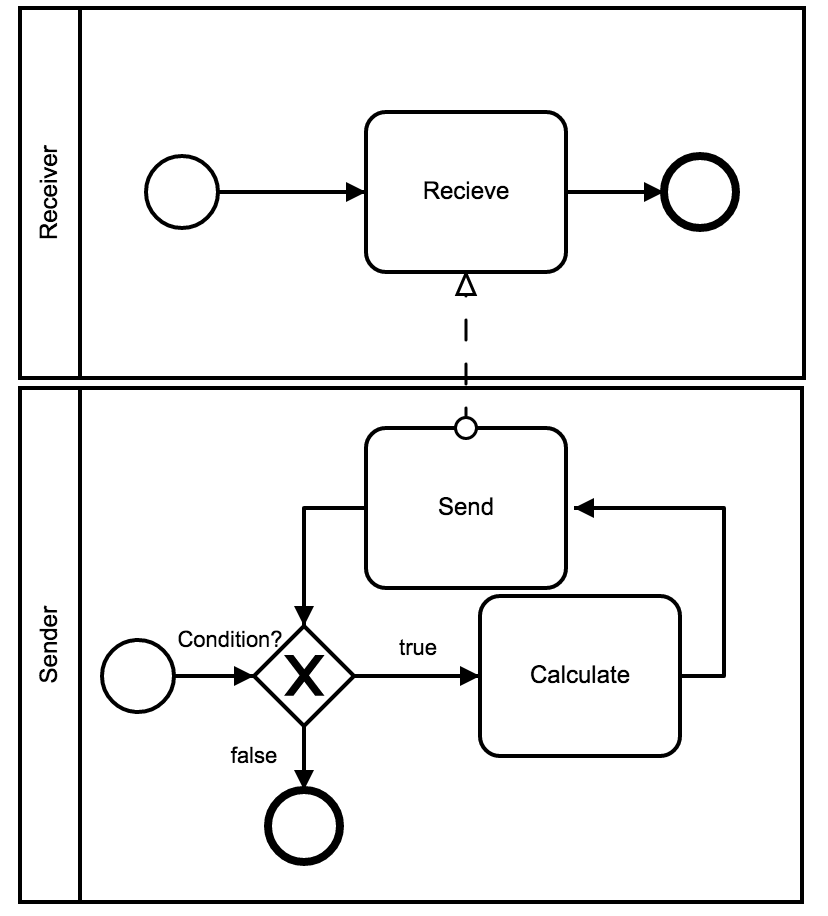
\includegraphics[width=43ex]{img/runningex.png}
\caption{An example of messaging in BPMN}
\label{fig:bpmnexvisa}
\end{figure}


The desired behavior of this model is that the processes start, the message exchange occurs, and they end. However, it is possible that the \emph{sender} process finishes without sending any message. In this case,  the \emph{receiver} process keeps waiting for a message that will never arrive. This is an example of \emph{deadlock}.

In addition, the model contains a \emph{livelock}, which occurs if after the \emph{receiver} process receives a message from the \emph{sender} process and finishes, the \emph{sender} keeps going back to the sending step and does not end.
\end{BehExample}

%Later, throughout this thesis, we show how our tools can help to detect such problems on the business process models. 
%???????????????????
